\subsection{Result 3}
Building on the Result 1 analysis, an additional entity - Sakai presence events - was taken into account, requiring configuration adjustments of nETL and CouchDB to aggregate across three entities instead of two entities. This analysis looks at the relationship between student benchmarks in the FU data and resultant course grades as a factor of Sakai usage. In other words, this analysis addresses the question of whether making more frequent use of the Sakai platform is shown to increase course performance for CSC1015F. However, the Sakai data - measured as presence events - cannot be associated with particular courses. As such the analysis takes into account only ``general usage'' of the Sakai LMS, and not usage of Sakai for these particular courses.

The nETL task configurations to load Grade data and FU data into CouchDB are mostly the same as the task configurations as used to achieve Result 1, except that Grade data is filtered to only include course results from 2016 via whitelisting (since Event data is only for 2016). A 3rd task is added to the configuration object to load the Event data into CouchDB. Configuration for nETL and CouchDB Map and List functions is included in the appendix (see \ref{netl-run3-config}, \ref{result-3-map} and \ref{result-3-list} respectively).

\subsection*{\textit{nETL} Event data configuration}
\begin{enumerate}
    \item Batches of 30 000 lines are extracted iteratively (and sequentially) as an array of lines (30 000 lines per batch seemed to be the sweetspot for what could be loaded into CouchDB's \textit{\_bulk\_docs} endpoint using nETL and still receiving optimal visual feedback in terms of continuous logging)
    \item Within each batch, each line is converted to a JSON object, transforming the batch into an array of objects. These objects each have the following fields: ``event\_date'', ``event\_id'', ``uct\_id'',  ``site\_key'', ``ref''
    \item The array of objects is filtered via whitelising objects on two fields: 1) ``uct\_id'' - only IDs of students who attended CSC1015F are considered. 2) ``event\_id'' - only the value ``281'' is considered, as these are representative of `presence' events
    \item A field is added to each object in the batch (``type\_'') and give the value ``vulaEvent''
    \item Superfluous object fields are removed via a whitelisting process, resulting in a batch (an array) of objects with the fields: ``event\_date'', ``event\_id'', ``uct\_id'', ``site\_key'', ``type\_''
    \item Each batch is loaded into CouchDB using the \textit{\_bulk\_docs} endpoint (as discussed previously), and the next batch is extracted on a success message from CouchDB
\end{enumerate}


\subsection*{The MapReduce function}
TODO

\begin{figure}[ht]
    \centering
    \begin{mdframed}
        \centering
        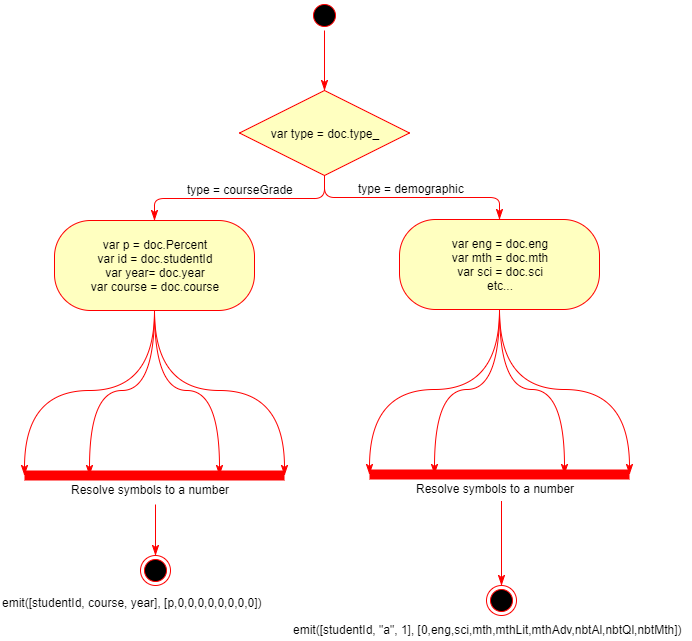
\includegraphics[scale=0.35]{./resources/figures/activity-diagram-1.png}
    \end{mdframed}
    \caption[Result 1 Map function]{\textbf{Figure \ref{result-3-map-fn}: Activity diagram showing logic Map function logic for Results 3 \& 4.}}
    \label{result-3-map-fn}
\end{figure}

\subsection*{The List function}
TODO